\section{Parameter Table}
Symbols that newly appear in this section are listed in table \ref{tab.symbol2}. Some of the symbols in table \ref{tab.symbol} are also used in this section and are not listed here.
\begin{table}[htbp]
             \centering
                \begin{tabular}{|l|l|}
                \hline
                Symbol & Defination \\
                \hline
                 $\mathcal{N}_i$ & total volume of population in city $i$\\

                $\mathcal{S}_i$ & number of susceptible people in city $i$\\

                $\mathcal{I}_i$ & number of infected but not segregated people in city $i$\\

                $\mathcal{G}_i$ & number of segregated and also infected people in city $i$\\

                $\mathcal{D}_i$ & number of death caused by EVD in city $i$\\

                $\mathcal{R}_i$ & number of recovered people (also immunized) in city $i$\\
                
                \textbf{$P_{i}$} & Total number of people in city $i$ apart from the people who are \\ & dead and segregated \\

                \textbf{$t_{i,j}$} & number of people transmit from city $i$ to city $j$ indeed \\

                \textbf{$\alpha$} & transmission coefficient \\

                \textbf{$d_{i,j}$} & distance from city $i$ to city $j$ \\
                
                $vacc_{tot}$ & the number of shares of vaccine that can be provided to all the cities every day\\
                
                $vacc_{i}$ & the number of shares of vaccine that can be provided to city $i$ every day\\
                \hline
                \end{tabular}
                \caption{The definition of the symbols.}  \label{tab.symbol2}
\end{table}

%%======================假设==================
%\subsection{Assumptions}
%\begin{itemize}
%  \item \textbf{People flow exists between any two cities }\\
%  Because no city would be quarantined totally in reality, there is connection between any two cities more or less, which means that there are flows of people between any two cities, although few people are flowing from one far-away small town to another.
%  \item \textbf{Cities are different}\\
%  To analyze the influence of delivery plan of medicines, it is better to consider that the population, location and initial status of each cities are different. To make our model realistic, we analyzed the last breakout of Ebola in west Africa in 2014 and chose some cities in the epidemic area. We consider information including geographic location, population of cities and distance between cities.
%  \item \textbf{Deterministic factors of people flow}\\
%  We assume that quantities of people leaving one city remains constant. Considering that the cities are laying on a 2-D plane, the intensity of people flow from one city to another is obviously inversely proportional to the distance between the two cities.
%  
%  We also assume that, for any individual, the probability of the one go out and link with (go to another city to visit friends, handle business affairs, etc.) any other individual are equal. Hence, it comes out that the people flow from one city to another is proportional to the product of populations of the two cities.

%  \item \textbf{Several properties of the system are time independent}\\
%To simplify our model, we assume that the quantities of drugs and vaccines delivered to each city per day are determined at the beginning and would not change with time. It means that the daily received quantity of drugs and vaccines for each city are constant. %This assumption is based on the engineering control program. Once the delivery plan has been decided, it would not change everyday because of too much sources wasting on the change.
%  
%We assume that the birth rate and natural mortality rate are generally equilibrium and fatality due to the disease is negligible compared with total population. It comes out that the total population (including fatality) is unchanging with time and the people flow among cities is also time independent.
%
%  \item \textbf{The segregated and dead would not transmit from one city to another}\\
%The S(Segregated) and D(dead due to the epidemic disease) are certainly not able to go from one city to another. Hence, when we calculated how many people from specific group are transmitted from one city to another, only the other three groups (the susceptible, the infected but not segregated, and the recovered and immunized) are taken into account.
%\end{itemize}

%\subsection{Construction of general model considering multiple cities}
%This model considering multiple cities are based on the previous single-city model. The difference between them is that in this multi-city model we consider the people flow among cities.
%
%Under assumptions previously mentioned, it is easy to conclude that the number of people transmitted from one city to another can be determined by 
%\begin{equation}
%t_{j,i} = t_{i,j}=\alpha \cdot\frac{1}{d_{i,j}}\cdot P_{i}\cdot P_{j}
%\end{equation}
%where
%\begin{equation}
%P_{i}=\mathcal{S}_{i}+\mathcal{I}_{i}+\mathcal{R}_{i}
%\end{equation}
%$\alpha$ is transmission coefficient which is a constant among all the cities, and $t_{i,j}$ is the number of people transmitted from city $i$ to city $j$.
%
%Different groups of people that are transmitted among cities are proportional to their proportion in departure city. Explicitly, for each day,
% \begin{align}\label{group}
%    \mathcal{S}_{j}&=\mathcal{S}_{j}+\sum_i \frac{\mathcal{S}_{i}}{P_{i}}\cdot t_{i,j}\\
%    \mathcal{I}{j}&=\mathcal{I}_{j}+\sum_i \frac{\mathcal{I}_{i}}{P_{i}}\cdot t_{i,j}\\
%    \mathcal{R}_{j}&=\mathcal{R}_{j}+\sum_i \frac{\mathcal{R}_{i}}{P_{i}}\cdot t_{i,j}
% \end{align}
% 
%Hence, previous derived difference equations can be written as
%\begin{subequations}
%\begin{align}
%  \dfrac{\mathcal{S}_{i+1} - \mathcal{S}_{i}}{\Delta t}&=-\frac{h}{\sigma}\mathcal{S}_i\mathcal{I}_i-\frac{vacc}{\sigma}+\sum_i \frac{\mathcal{S}_{i}}{P_{i}}\cdot t_{i,j}\\
%  \dfrac{\mathcal{I}_{i+1} - \mathcal{I}_{i}}{\Delta t}&=\frac{h}{\sigma}\mathcal{S}_i\mathcal{I}_i-\frac{(k_1+g+r_s)}{\sigma}\mathcal{I}_i+\sum_i \frac{\mathcal{I}_{i}}{P_{i}}\cdot t_{i,j}\\
%  \dfrac{\mathcal{G}_{i+1} - \mathcal{G}_{i}}{\Delta t}&=\frac{g}{\sigma}\mathcal{I}_i-\frac{k_2}{\sigma} \mathcal{G}-\frac{r_g}{\sigma} \mathcal{G}\\
%  \dfrac{\mathcal{R}_{i+1} - \mathcal{R}_{i}}{\Delta t}&=\frac{r_s}{\sigma}\mathcal{I}_i+\frac{r_d}{\sigma} \mathcal{G}_i+\sum_i \frac{\mathcal{R}_{i}}{P_{i}}\cdot t_{i,j}\\
%  \dfrac{\mathcal{D}_{i+1} - \mathcal{D}_{i}}{\Delta t}&=\frac{k1}{\sigma}\mathcal{I}_i+\frac{k_2}{\sigma} \mathcal{G}_i
%\end{align}
%\end{subequations} 
% 
%\subsection{Numerical Computation of general model considering multiple cities}
%At first, we exam the multi-city model with a simplified situation in which the quantities of drugs and vaccines delivered to each city are the same. We will show that it properly figures out the general trend of the spread of disease among cities and show us some significant character of the process.
%\subsubsection{Process of numerical computation}
%The steps of calculation are listed below:
%\begin{enumerate}
%  \item \textbf{Initial conditions}
%  \item \textbf{Calculation based on single-city model for each city }
%  \item \textbf{Simulate people flows among cities}
%  \item \textbf{Repeat Step 2 and Step 3 for the next moment}
%  \item \textbf{Until the preset $days$}
%\end{enumerate}
%In fact, from single-city model to multiple-city model, we simply added step 3.
%
%Other parameters that we are used in the computation, if not stated specifically, are the same as single-city model. For clarity, we also list them here.
%
%$\beta = 0.32$ , $k_1 = 0.023$, $r_s = 0.0103$ , $days = 150$ ,  $\Delta t = 0.1 (\text{days})$.
%
%\subsubsection{Selection of geographic data}
%Since the outbreak of EVD are usually constrained in regional areas (mentioned in background), the geographic data that we selected to simulate the last break of EVD is all from the three countries in west Africa (Guinea, Liberia and Sierra Leone). There are 145 cities in these three countries (geographic locations are plotted in figure \ref{allcity}). If all taken into account, it is not only beyond the computational ability of our computers, but also, even if results are given, is difficult for us to study the details of the results. Hence, we select 18 representative cities, among which there are big cities and also small towns; there are cities that are close to each other and there are cities far away. The data of the selected 18 cities are listed in table \ref{citylist}. For the convince of later analysis, a visualized version of data of the cities are ploted in figure \ref{cityplot}. 
%
%\begin{figure}
%\centering
%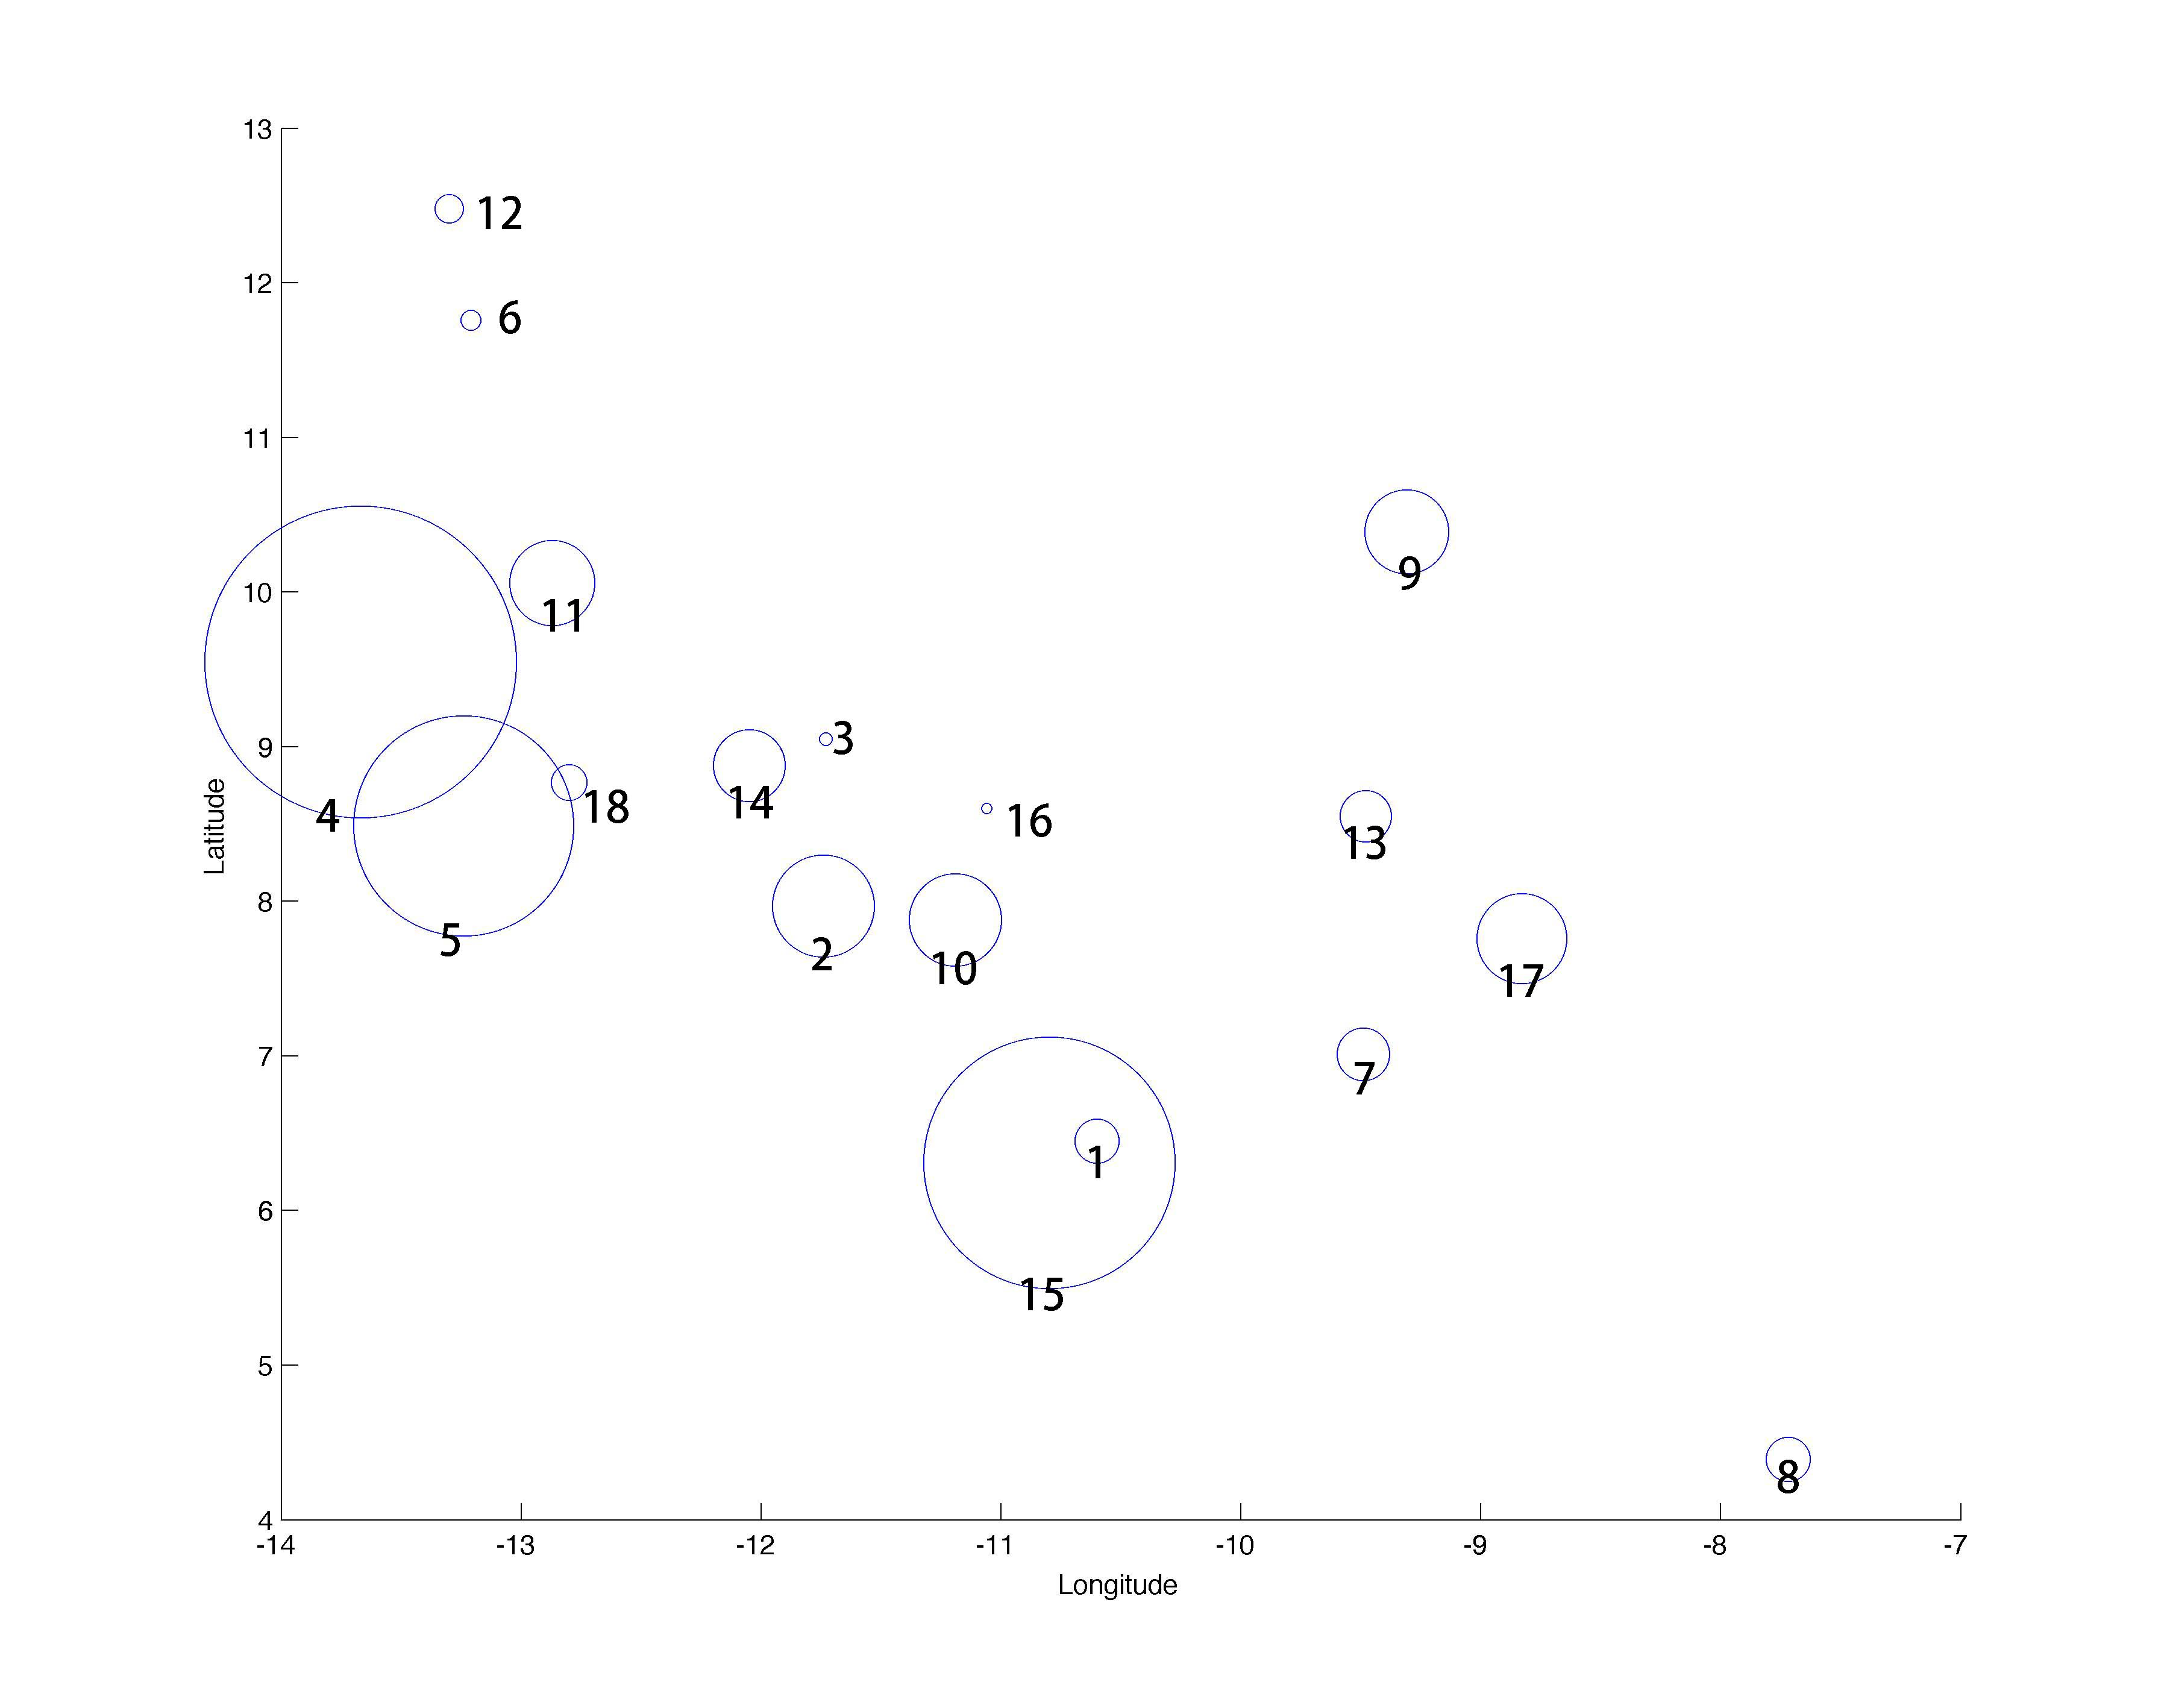
\includegraphics[width = 0.8\textwidth]{CityPopulationlabel.jpg}
%\caption{Information of 18 selected cities. Each circle stands for a city - the center of circle stands for location and the area of circle stands for population. The labels on or nearby the circles are corresponding to the labels in table \ref{citylist}}
%\label{cityplot}
%\end{figure}
%
%\begin{figure}
%\centering
%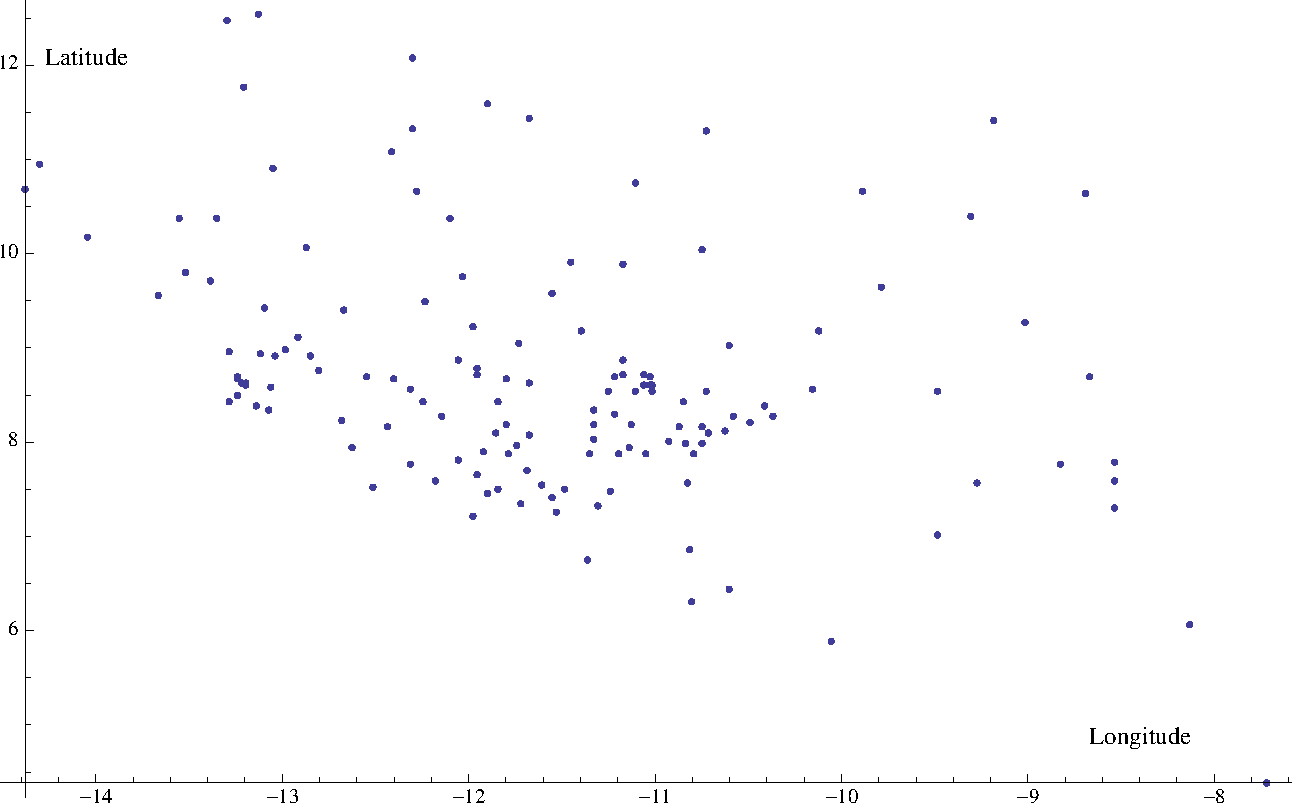
\includegraphics[width = 0.6\textwidth]{allcity.pdf}
%\caption{Locations of cities in the three countries}
%\label{allcity}
%\end{figure}
%
%\begin{table}[htb]
%\centering
%\begin{tabular}{|r|r|r|r|r|r|r|}
%    \hline
%    Label & City & Province/Region & Country & Latitude & Longitude & Population \\
%    \hline
%1 & \text{Bensonville} & \text{Montserrado} & \text{Liberia} & 6.45 & -10.6 & 33188 \\
%2& \text{Bo} & \text{Southern} & \text{SierraLeone} & 7.97 & -11.74 & 167144 \\
%3& \text{Bumbuna} & \text{Northern} & \text{SierraLeone} & 9.05 & -11.73 & 3222 \\
%4& \text{Conakry} & \text{Conakry} & \text{Guinea} & 9.55 & -13.67 & 1548470 \\
%5& \text{Freetown} & \text{Western} & \text{SierraLeone} & 8.49 & -13.24 & 772873 \\
%6&\text{Gaoual} & \text{Gaoual} & \text{Guinea} & 11.76 & -13.21 & 7461 \\
%7& \text{Gbarnga} & \text{Bong} & \text{Liberia} & 7.01 & -9.49 & 45835 \\
%8& \text{Harper} & \text{Maryland} & \text{Liberia} & 4.39 & -7.72 & 32661 \\
%9& \text{Kankan} & \text{Kankan} & \text{Guinea} & 10.39 & -9.31 & 114009 \\
%10& \text{Kenema} & \text{Eastern} & \text{SierraLeone} & 7.88 & -11.19 & 137696 \\
%11& \text{Kindia} & \text{Kindia} & \text{Guinea} & 10.06 & -12.87 & 117062 \\
%12& \text{Koundara} & \text{Koundara} & \text{Guinea} & 12.48 & -13.3 & 13990 \\
%13& \text{Macenta} & \text{Macenta} & \text{Guinea} & 8.55 & -9.48 & 43102 \\
%14& \text{Makeni} & \text{Northern} & \text{SierraLeone} & 8.88 & -12.05 & 85017 \\
%15& \text{Monrovia} & \text{Montserrado} & \text{Liberia} & 6.31 & -10.8 & 1010970 \\
%16& \text{Ndoyogbo} & \text{Eastern} & \text{SierraLeone} & 8.6 & -11.06 & 1870 \\
%17& \text{Nzerekore} & \text{Nzerekore} & \text{Guinea} & 7.76 & -8.83 & 132728 \\
%18& \text{PortLoko} & \text{Northern} & \text{SierraLeone} & 8.77 & -12.8 & 21961 \\
% \hline
%\end{tabular}
%\caption{Information of the 18 selected cities}
%\label{citylist}
%\end{table}
%
%\subsubsection{Results of numerical computation}
%Similarly, we observed both outbreak situations and well-controlled conditions when we change any one of the four independent variables($g$, $drug$, $vacc$ and $C$).
%
%Figure \ref{multibreak} shows clearly how the outbreak of disease spread from one city to another. We have observed that: 1) the order of severity (measured by fatality) is larger in the city which is the onset of disease (in our special case it is city 1) ; 2) epidemic outbreak occurs earlier in the city which is the onset of disease, in another word, the general trend of others has somewhat 'lag effect'; 3) the general trend of the city close to the onset of disease resembles more to the onset of disease in terms of severity and time sequence (in our special case it is city 15).
%
%\begin{figure}
%\centering
%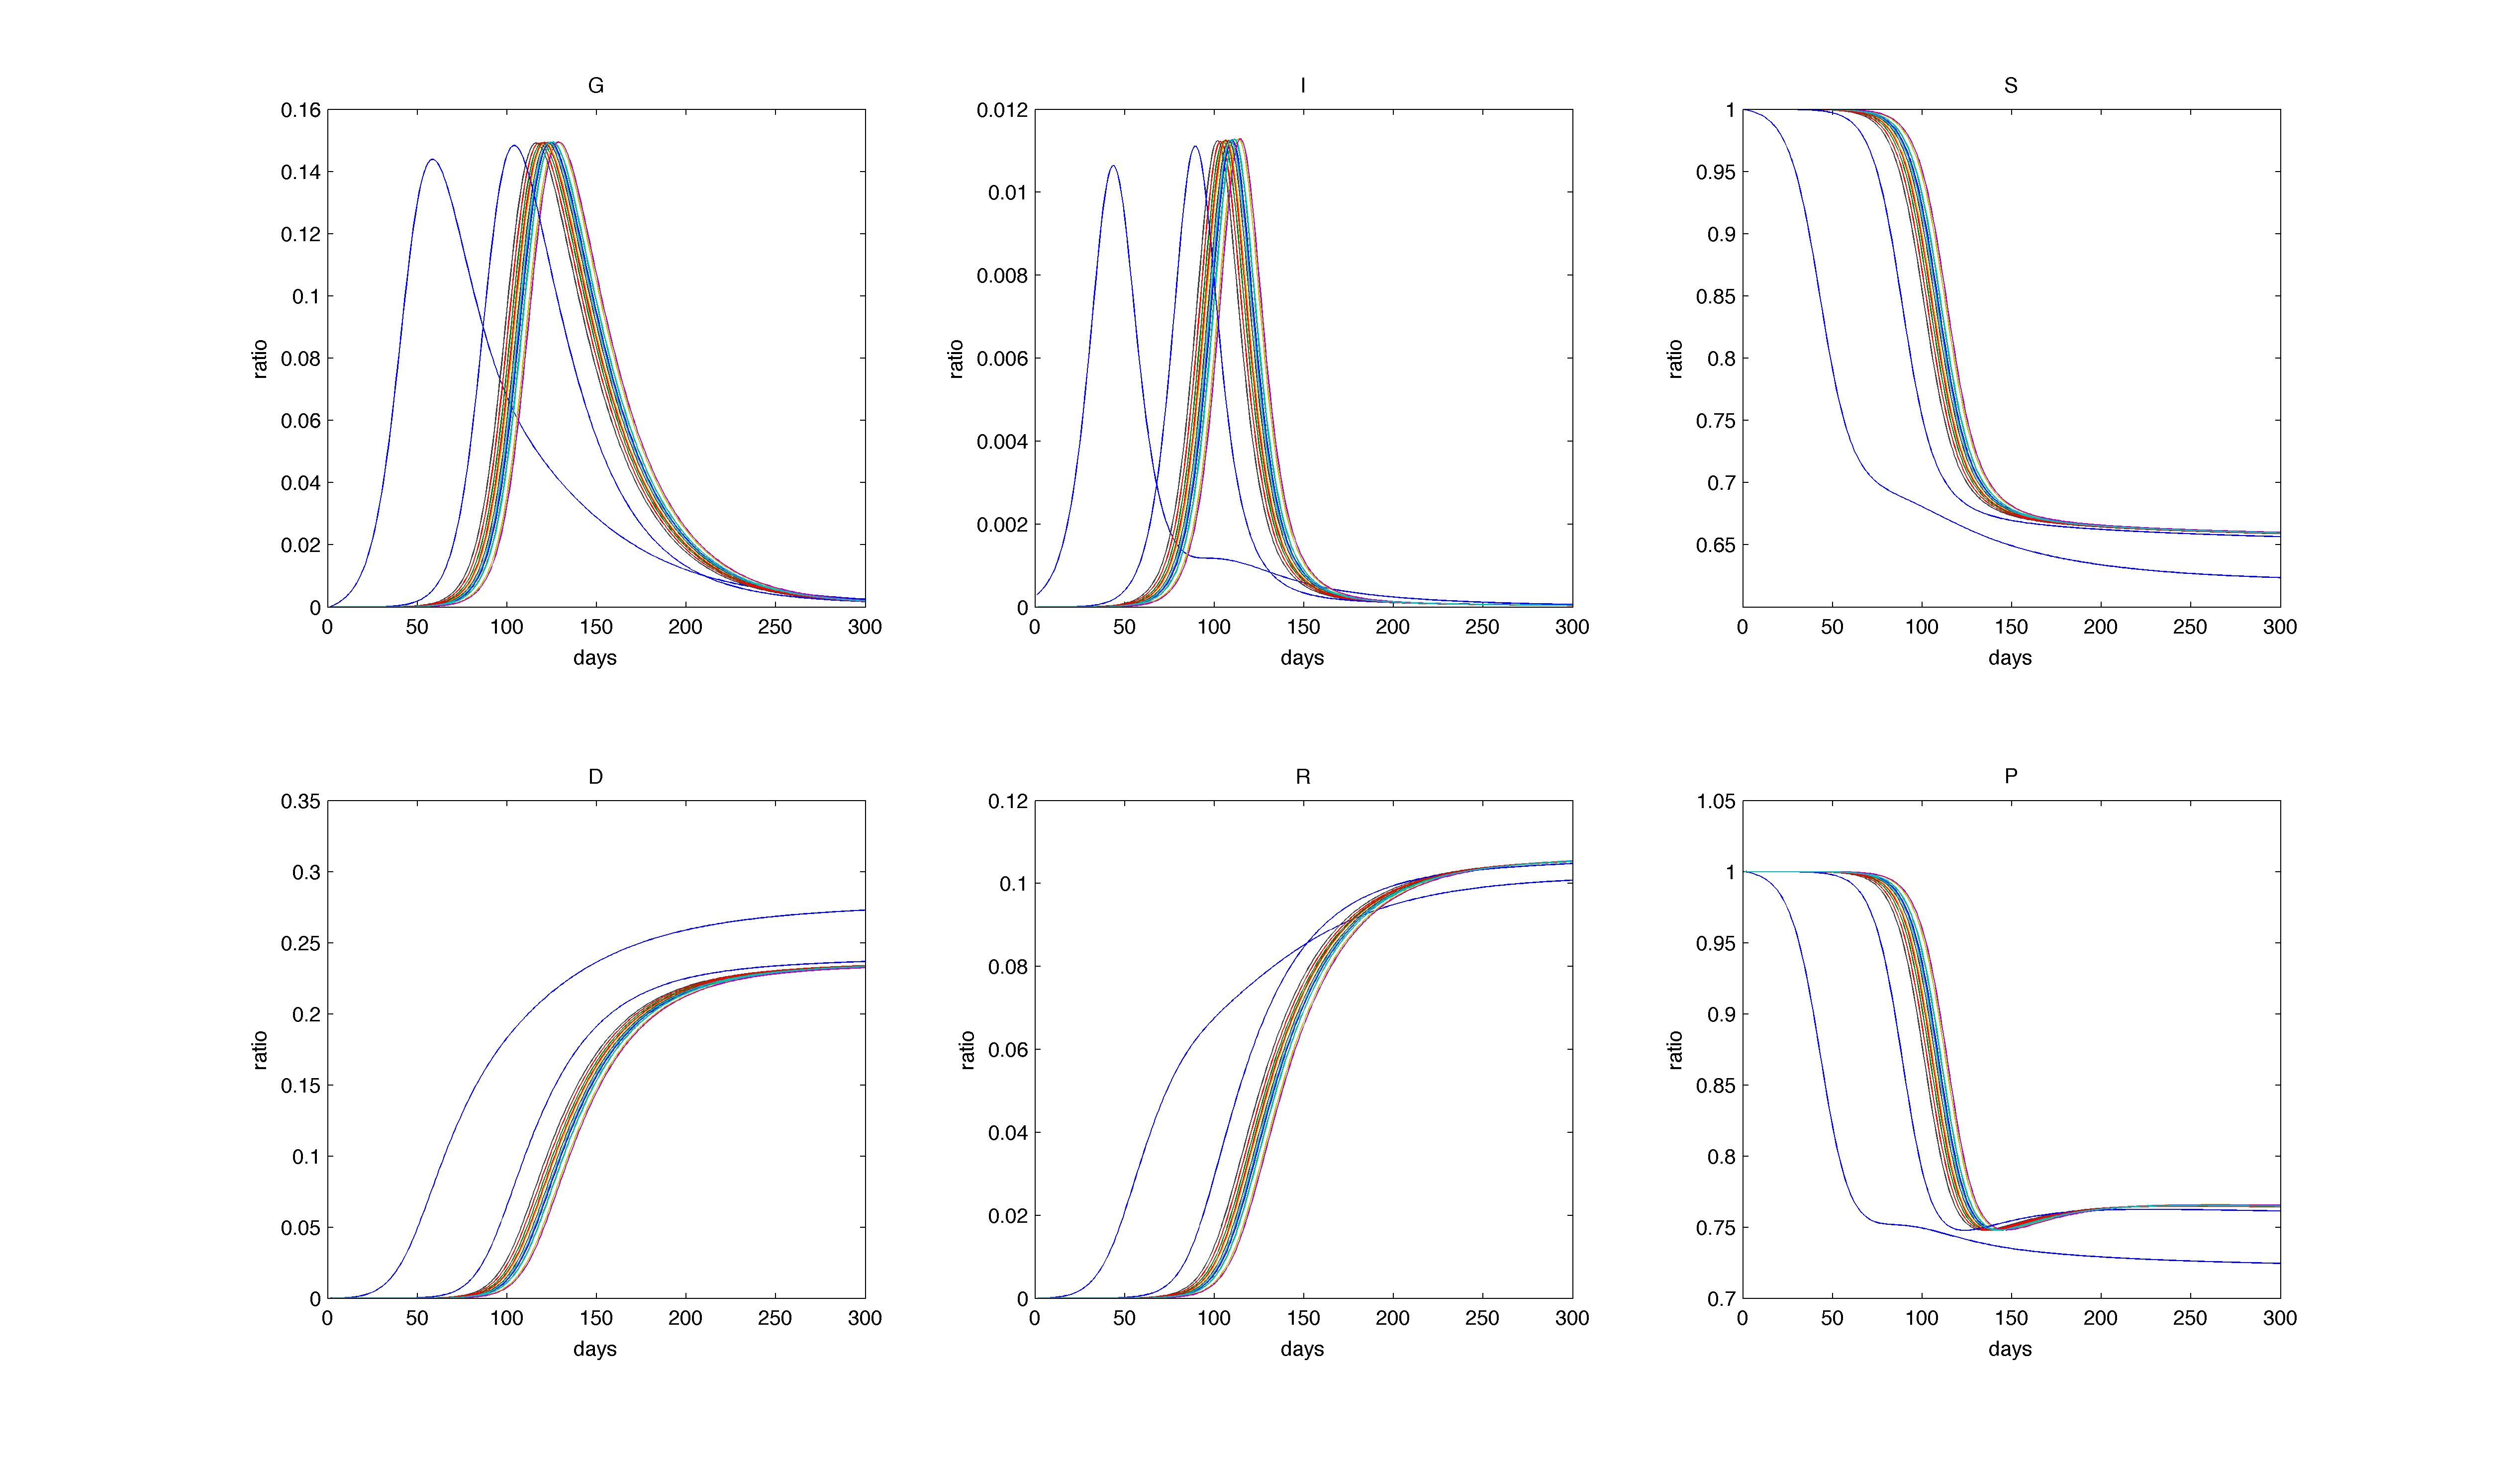
\includegraphics[width = 0.8\textwidth]{multibreak.jpg}
%\caption{epidemic disease breakout in different cities. $days = 300$, $\alpha = 10^{-4}$ , $drug = 0, vacc = 0, C = 3, g = 0.8$ and the y axis is the number of people in the group divided by the total number of people in corresponding city. Initially, 10 people are infected in city 1, and all the other people in all the cities are susceptible. The dark blue line far away from others represents city 1. The next dark blue line which is easy to distinguish from others represents city 15 which is geographically close to city 1.}
%\label{multibreak}
%\end{figure}
%
%Figure \ref{multicontrol_1000vacc} shows that when giving vaccines to the cities, the severity greatly decreases, which indicates the great influence medication has on the spread of disease. Additionally, we have observed a new phenomenon that big cities are more easy to get influenced by epidemic diseases if all the cities are given identical amount of drug or vaccine. In our special case, the trend of city 4 is showing the phenomenon. Similar features are observed when varying the value of $drug$, $C$, or $g$.
%
%\begin{figure}
%\centering
%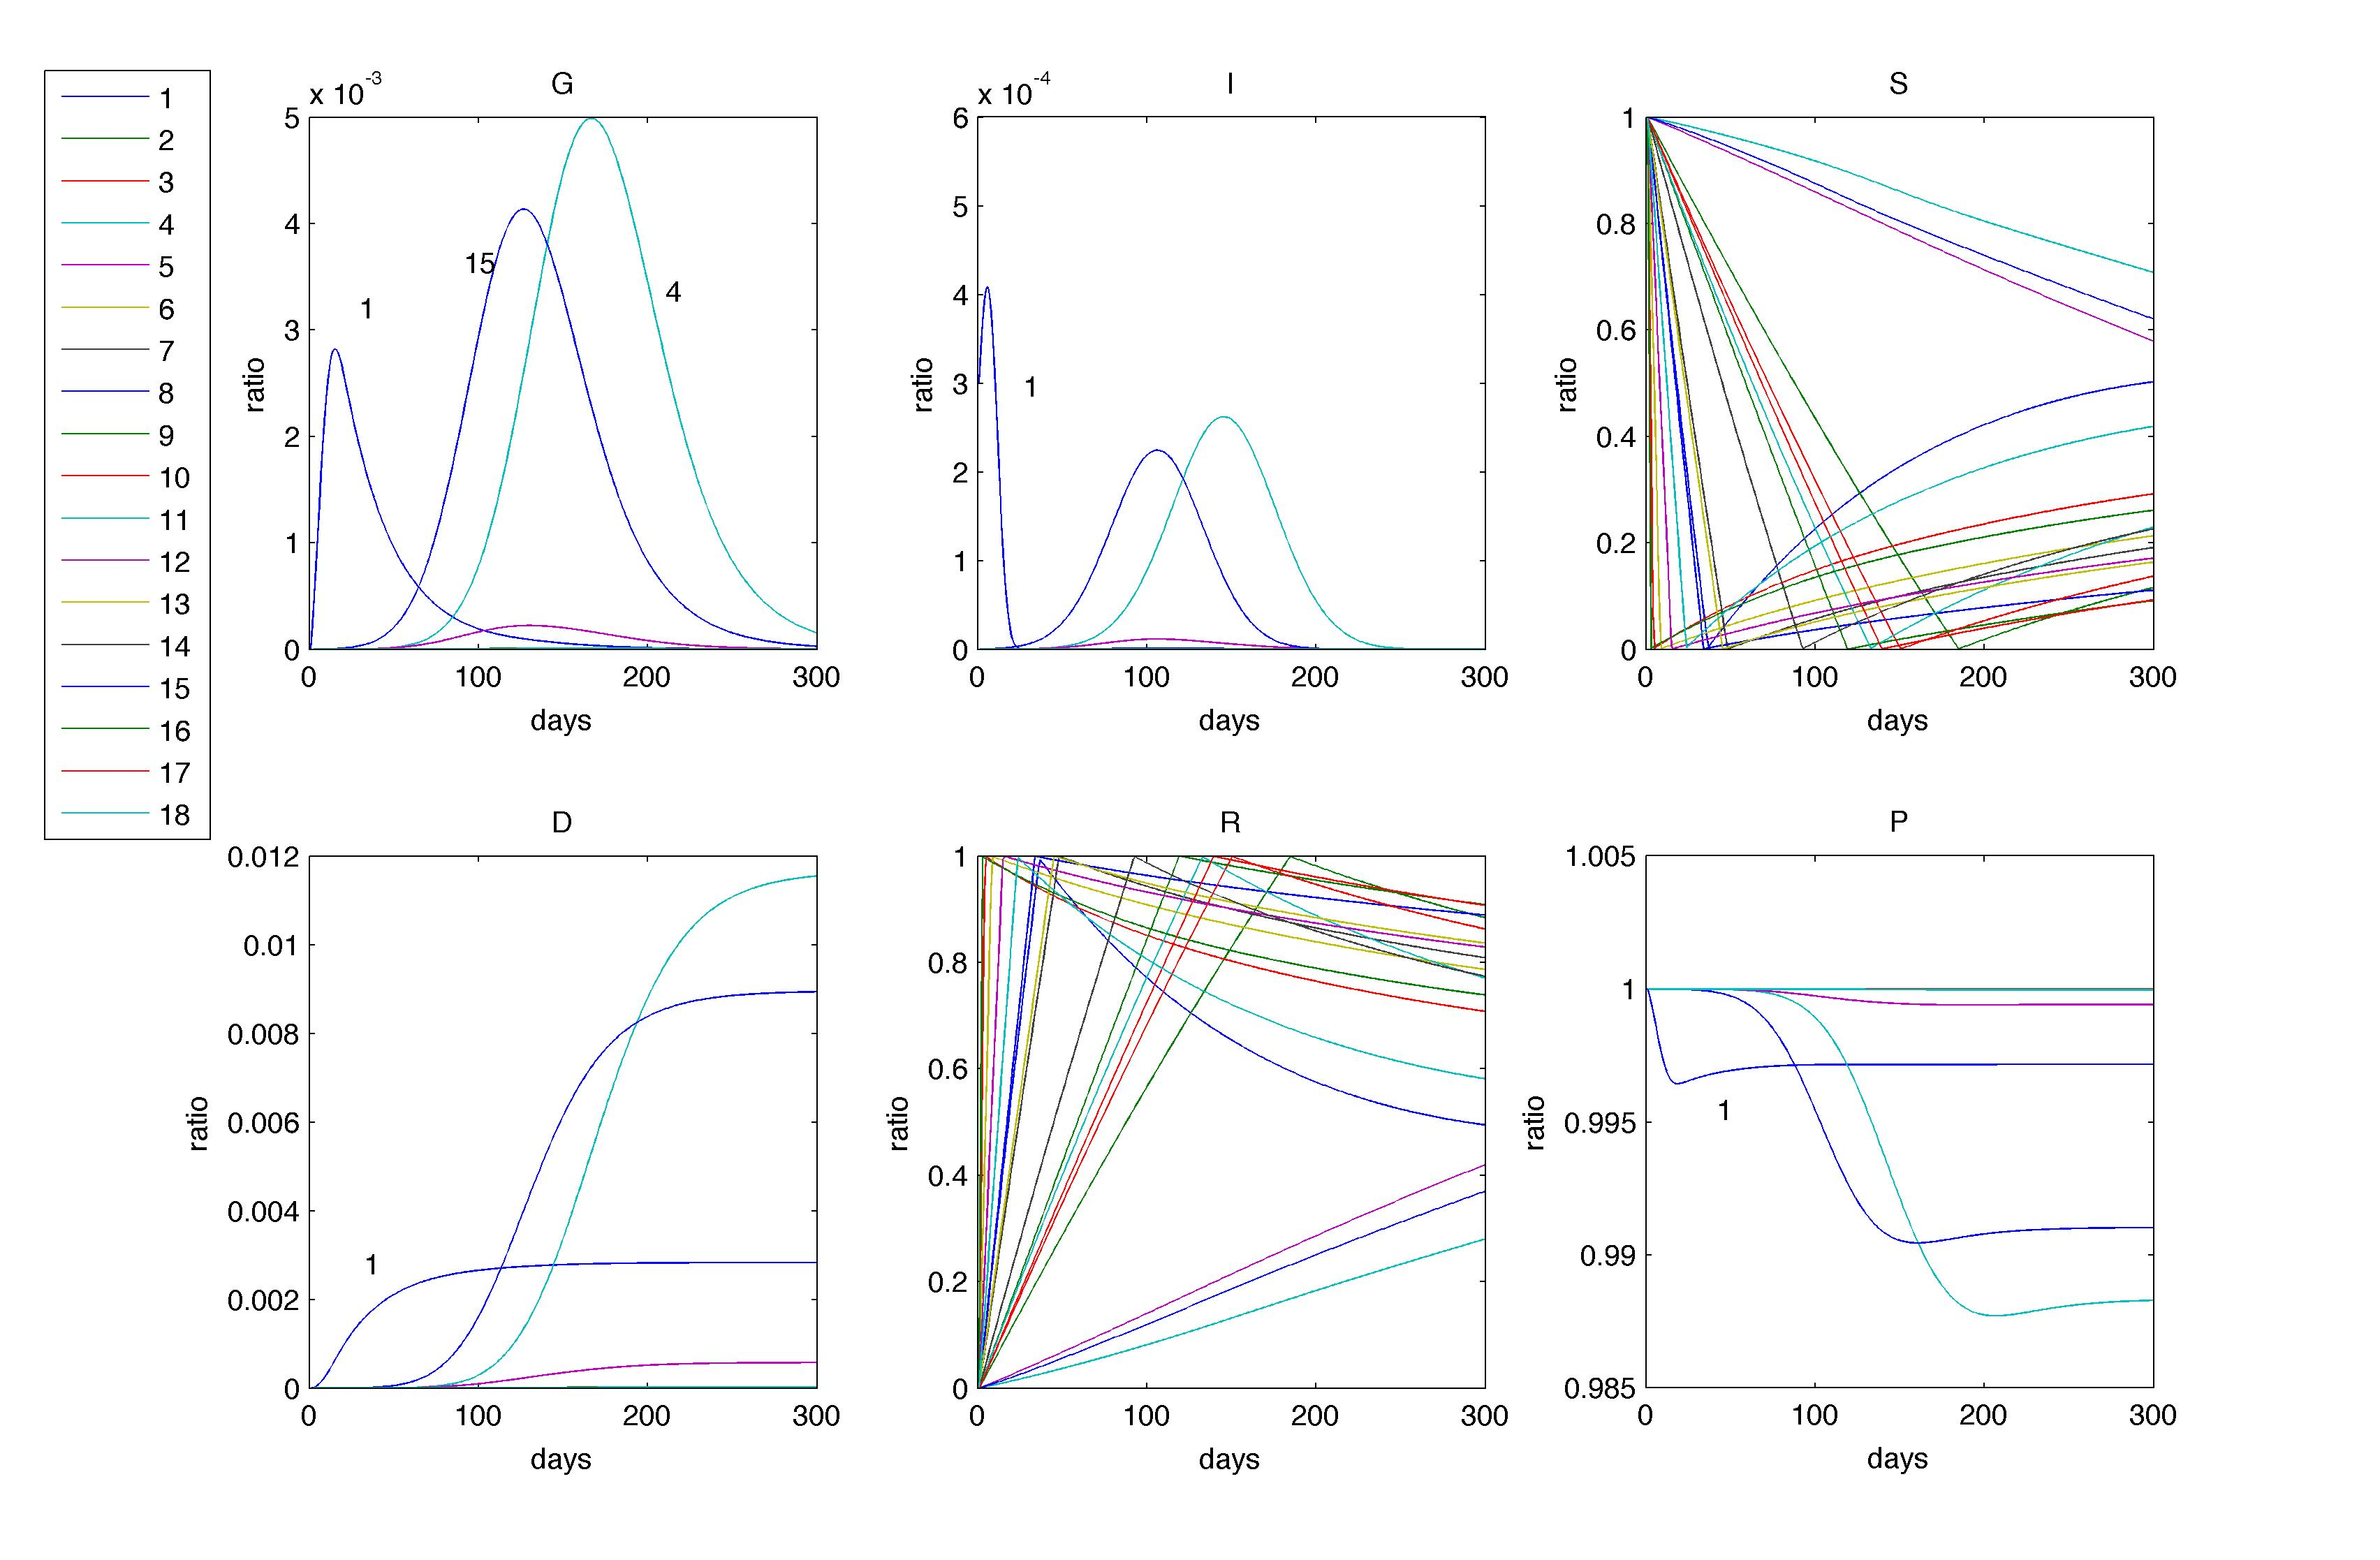
\includegraphics[width = 0.8\textwidth]{multicontrol_1000vacc.jpg}
%\caption{epidemic disease breakout in different cities. $days = 300$, $\alpha = 10^{-4}$ , $drug = 0, vacc = 1000, C = 3, g = 0.8$ and the y axis is the number of people in the group divided by the total number of people in corresponding city. Initially, 10 people are infected in city 1, and all the other people in all the cities are susceptible. The dark blue with label '1' represent city 1. The other dark blue line represents city 15 which is geographically close to city 1. The light green line with label '4' represent city 4 which is the biggest city in the all 18 cities.}
%\label{multicontrol_1000vacc}
%\end{figure}
%
%The observed phenomenon also indicates that some of the cities need more medications than the others. Hence, a carefully organized plan to delivery drugs and vaccines is needed, which will be discussed next.
%
%\subsection{Model for optimizing the medication plan}
%We have seen that different medication plans (the plans to allocate drugs and vaccines) can influence the severity of the spread of disease (measured by the total death due to the disease). Hence, here comes the question: how can we develop a plan that can reduce the number of death as much as possible.
%
%Let us first consider a practical problem where the amount of vaccine that can be provided every day is a constant $vacc_{tot}$ (in the later computation we set the value to $vacc_{tot} = 1800$), and we are required to find out a plan to allocate the vaccines in order that the total death is as small as possible.
%\subsubsection{Genetic algorithm}
%Since there are many degrees of freedom of the possible plans, it is justifiable for us to use optimization algorithm to solve the problem. In order to use genetic algorithm, which is one of the most effective optimization algorithm, it is required that the degree of freedom of the plan which is to be optimized should be encoded into the form of binary `chromosome`. We encoded them into a 180-bit chromosome which is illustrated in figure \ref{chromosome}. The 180-bit chromosome is divided into 18 segments, each of which is representing the amount of vaccines that can be allocated to a city. The length of each segment representing a single city is $chromoUnitLength=10$, which is capable of donating value from 0 to $2^{10}-1$. We may as well donate the value of city $i$ as $w_i$, Hence, we can decide the amount of vaccines each city can get. The number of shares of vaccines that city $i$ can get per day is 
%\begin{equation}
%vacc_i = \dfrac{w_i}{\sum_{j=1}^{18} w_j} vacc_{tot}
%\end{equation}
%
%\begin{figure}
%\centering
%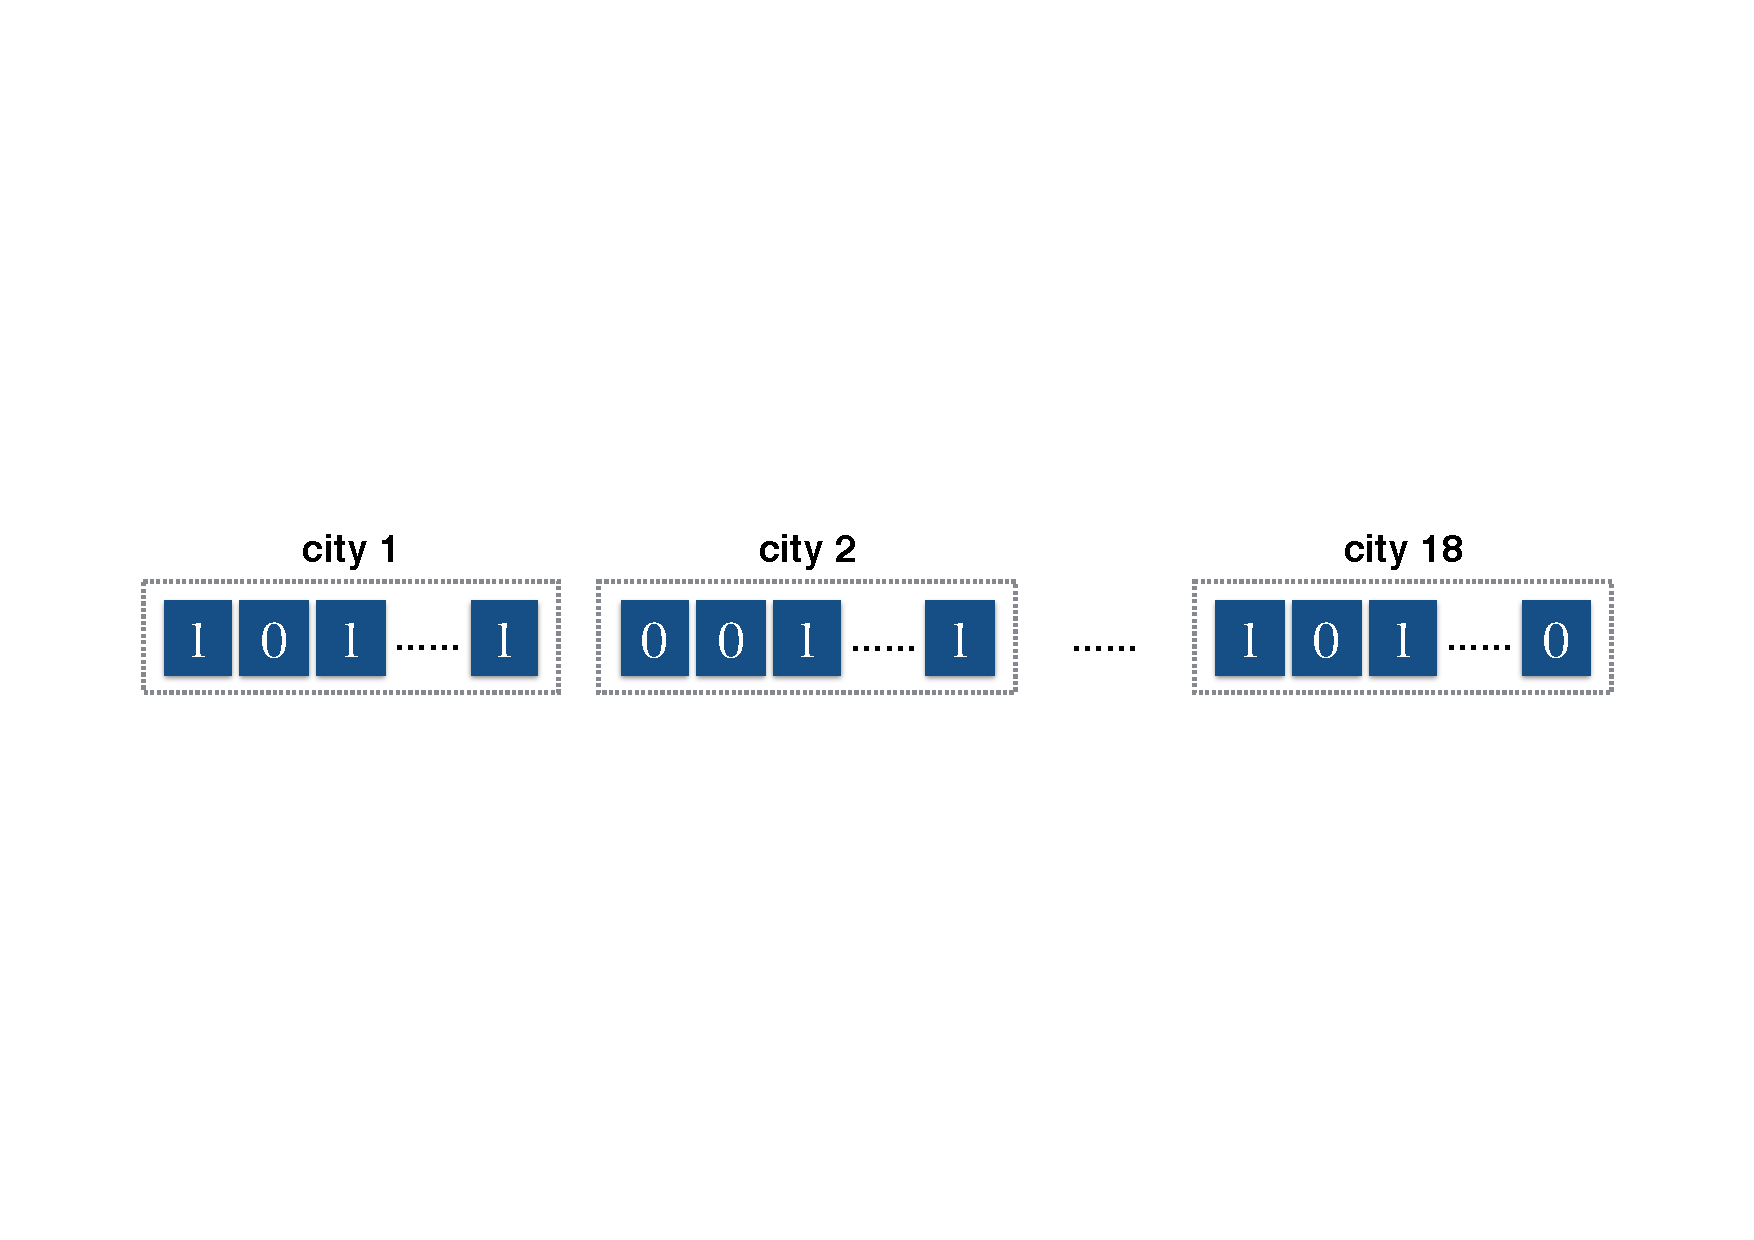
\includegraphics[width = \textwidth]{chromosome.pdf}
%\caption{Encoding}
%\label{chromosome}
%\end{figure}
%
%The process of genetic algorithm we adopted are shown in figure \ref{GA}.
%
%On the stage of initialization (step 1 labeled in the figure), we set the number of generations to be calculated to $generationNum = 1000$, the number of individuals in each generation to $popSize = 200$, the rate of mutation to $mutationRate = 0.01$ and the rate of crossover to $crossoverRate = 0.6$.
%
%On the stage of calculating fitness (step 2), we set the fatality rate as the target function and take it as the value of fitness.
%
%The stage of selecting, crossover and mutation (step 3,4 and 5) are conform the very classic process of genetic algorithm.
%
%\begin{figure}
%\centering
%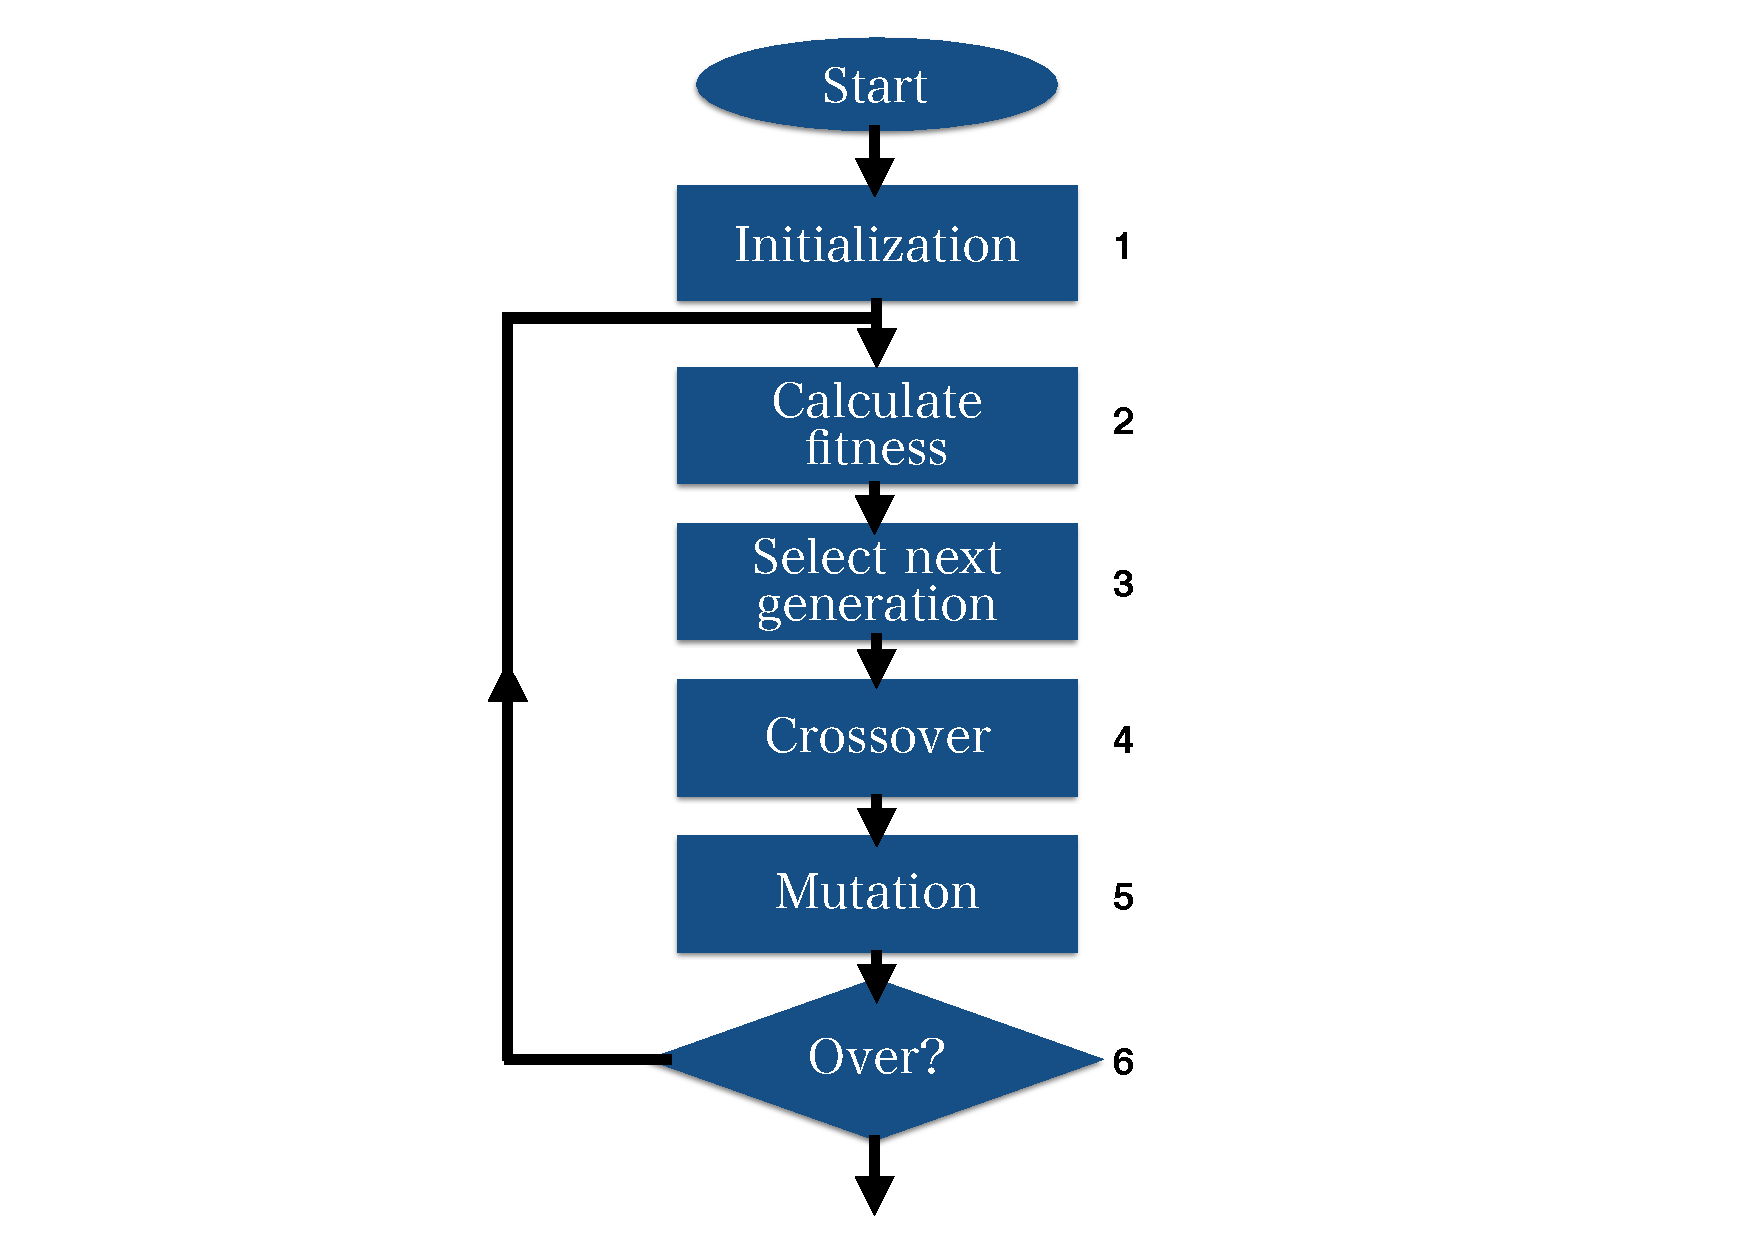
\includegraphics[width = 0.6\textwidth]{GA.pdf}
%\caption{The process of genetic algorithm}
%\label{GA}
%\end{figure}
%
%\subsubsection{Results of computation}
%With parameters shown in table \ref{comppara}. A optimized result is given by our program, which is shown in table \ref{result}. 
%
%The number of death declined from 2768 with randomly generated plan to 380 with the optimized plan shown in table \ref{result}. The declining trend can be easily seen in figure \ref{fitness_avg}.
%
%\begin{table}[]
%\centering
%\begin{tabular}{ccccccccc}
%\hline
%$\beta$ &$k_1$      &$r_s$  &$days$ &$\Delta t$ &$g$    &$C$    &$drug$ & number of initial infected people\\
% 0.32   &0.023      &0.0103 &150    &0.1        &0.8    &3  &0 & 10(in city 1)\\
%\hline
%\end{tabular}
%\begin{tabular}{cccccc}
%\hline
%$vacc_{tot}$&$chromoUnitLegth$ & $generationNum$ &$popSize$  &$mutationRate$ &$crossoverRate$ \\
%1800 &10 &1000            &200        &0.01           &0.6 \\
%\hline
%\end{tabular}
%\caption{Parameters in computation}
%\label{comppara}
%\end{table}
%
%\begin{table}[]
%\centering
%\begin{tabular}{|r|r|r|r|}
%\hline
%label of city&$vacc_i$&population of city & vaccine per capita ($\times 10^{-3}$)\\ \hline
%1&32&33190&0.96983\\ \hline
%2&367&167100&2.1956\\ \hline
%3&3&3222&0.9082\\ \hline
%4&315&1548000&0.20345\\ \hline
%5&185&772900&0.23947\\ \hline
%6&55&7461&7.4029\\ \hline
%7&40&45840&0.86178\\ \hline
%8&14&32660&0.41439\\ \hline
%9&31&114000&0.26952\\ \hline
%10&98&137700&0.71456\\ \hline
%11&41&117100&0.34673\\ \hline
%12&94&13990&6.7195\\ \hline
%13&24&43100&0.55164\\ \hline
%14&48&85020&0.5679\\ \hline
%15&329&1011000&0.32562\\ \hline
%16&51&1870&27.1889\\ \hline
%17&27&132700&0.20398\\ \hline
%18&47&21960&2.132\\ \hline
%\end{tabular}
%\caption{A optimized plan for allocating vaccine with $vacc_{tot} = 1800$ }
%\label{result}
%\end{table}
%
%\begin{figure}
%\centering
%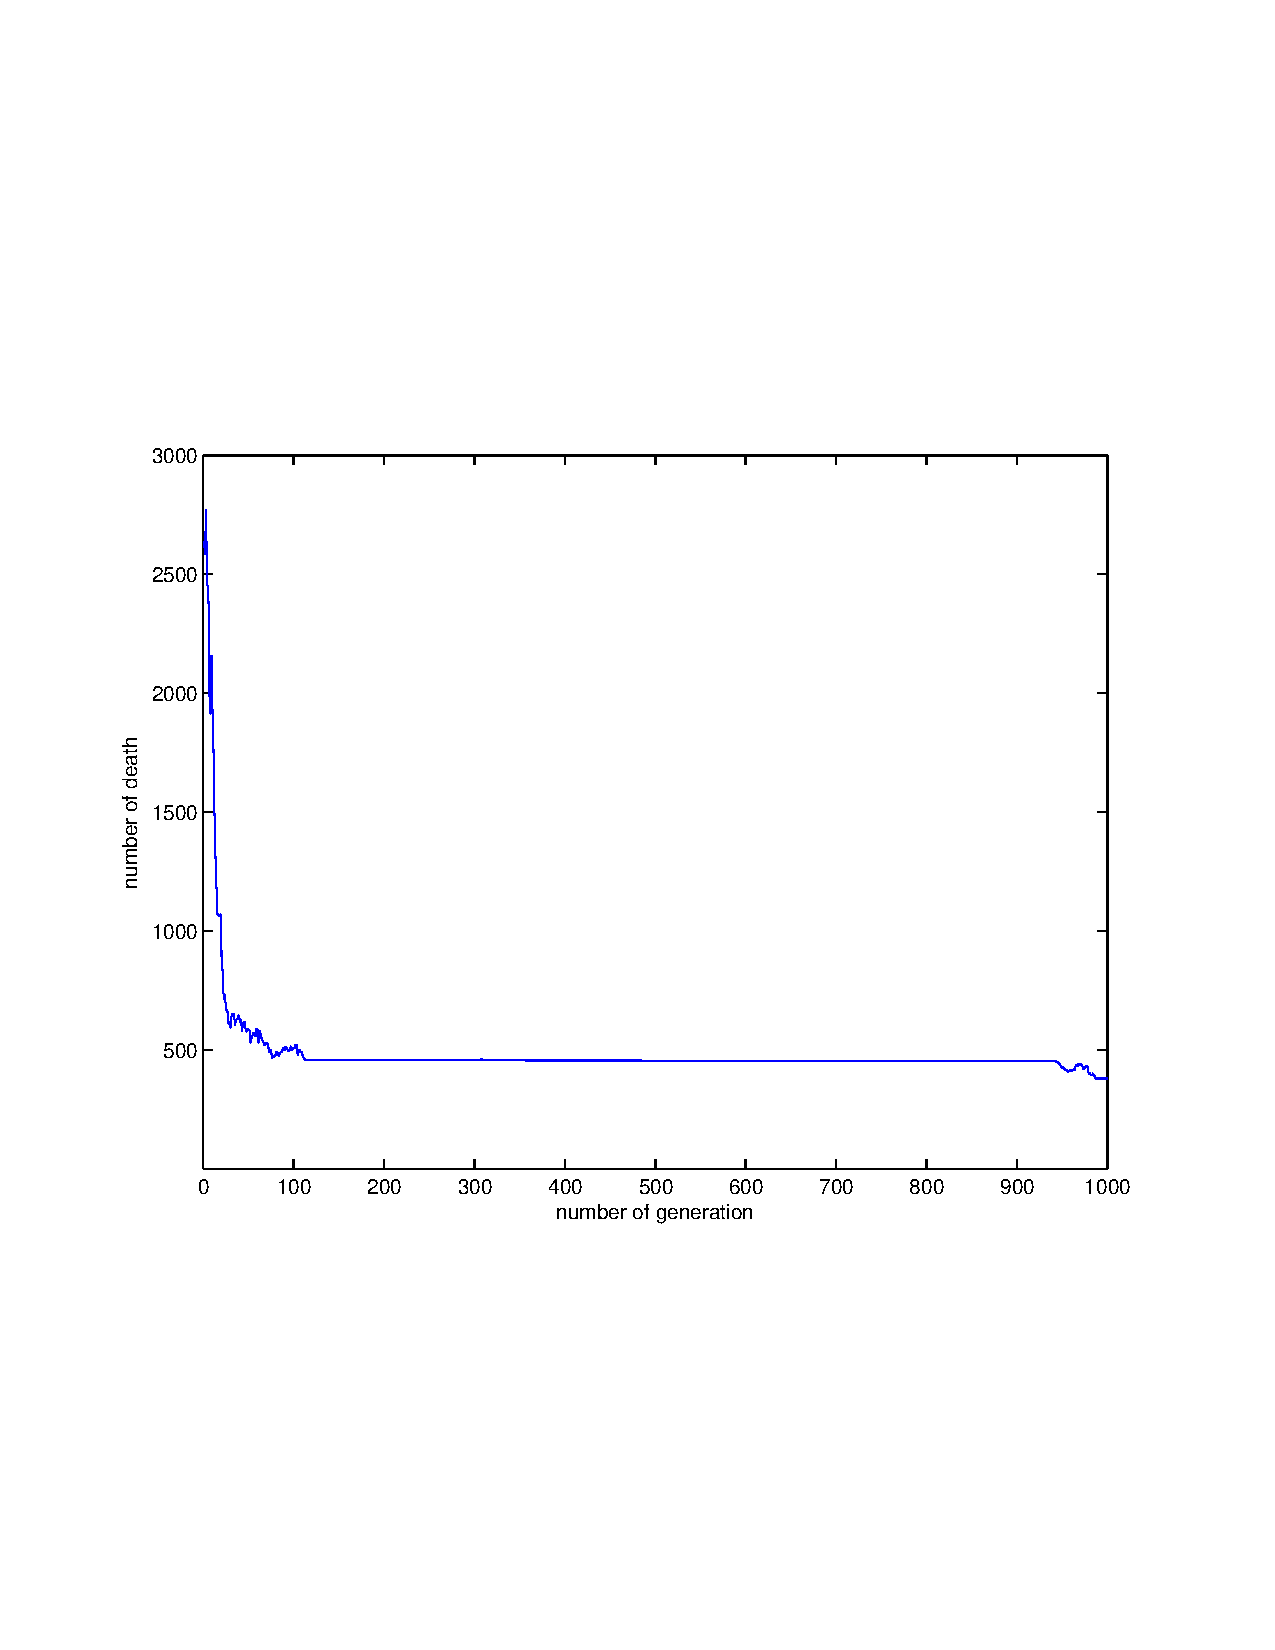
\includegraphics[width = 0.6\textwidth]{fitness_avg.pdf}
%\caption{The number of death declines with the optimization of the plan. The x axis is for the number of generations of genetic algorithm and the y axis is for the number of death in all the 18 cities.}
%\label{fitness_avg}
%\end{figure}
%
%\subsubsection{Analysis of the result}
%The result is analyzed from following aspects.
%\begin{enumerate}
%\item The two biggest cities - city 4 and city 15 - are allocated for more than 300 shares of vaccines, which is remarkably more than others. This outcome is easy to understand. The more people in the city, the more shares of vaccine are needed.
%\item Some of cities are allocated more shares of vaccine compared with their population, where city 16 is a significant example. City 16 is a small town, but it has the largest amount of vaccine per capita. It is easy to understand considering the geographic location of city 16. City 16 lies in the center of the cities we selected, which plays a significant role in the transmission of pathogen from one city to another. Once huge amount of vaccine is delivered to this city, the route of transmission of pathogen is greatly cut off.
%
%That the city near the center of network needs more vaccine per capita is clearly shown in figure \ref{vaccine_per_capita.pdf}.
%\item The largest amount of vaccine is allocated to city 2, which is a relatively big city and locates relatively in the center of all the cities, confirming the previous inference.
%\item Since people flow is supposed to be determined by the distances between cities, the amount of vaccine per capita is related to geographic location of cities. In real practice, the people flow is determined by more factors, such as convenience of traffic, so it is not difficult to imagine that \textbf{the cities that lie in the center of people flow network need larger amount of vaccine and drug per capita}.
%\item The computation above is varying the delivery plan for vaccine when the plan for drug is invariant. When the delivery plan for vaccine is invariant, the optimized delivery plan for drug has similar characteristics. Hence, we just list the mere optimized plan for drug in table \ref{drug} and are not repeating the similar interpretation.
%\end{enumerate}
%
%\begin{figure}
%\centering
%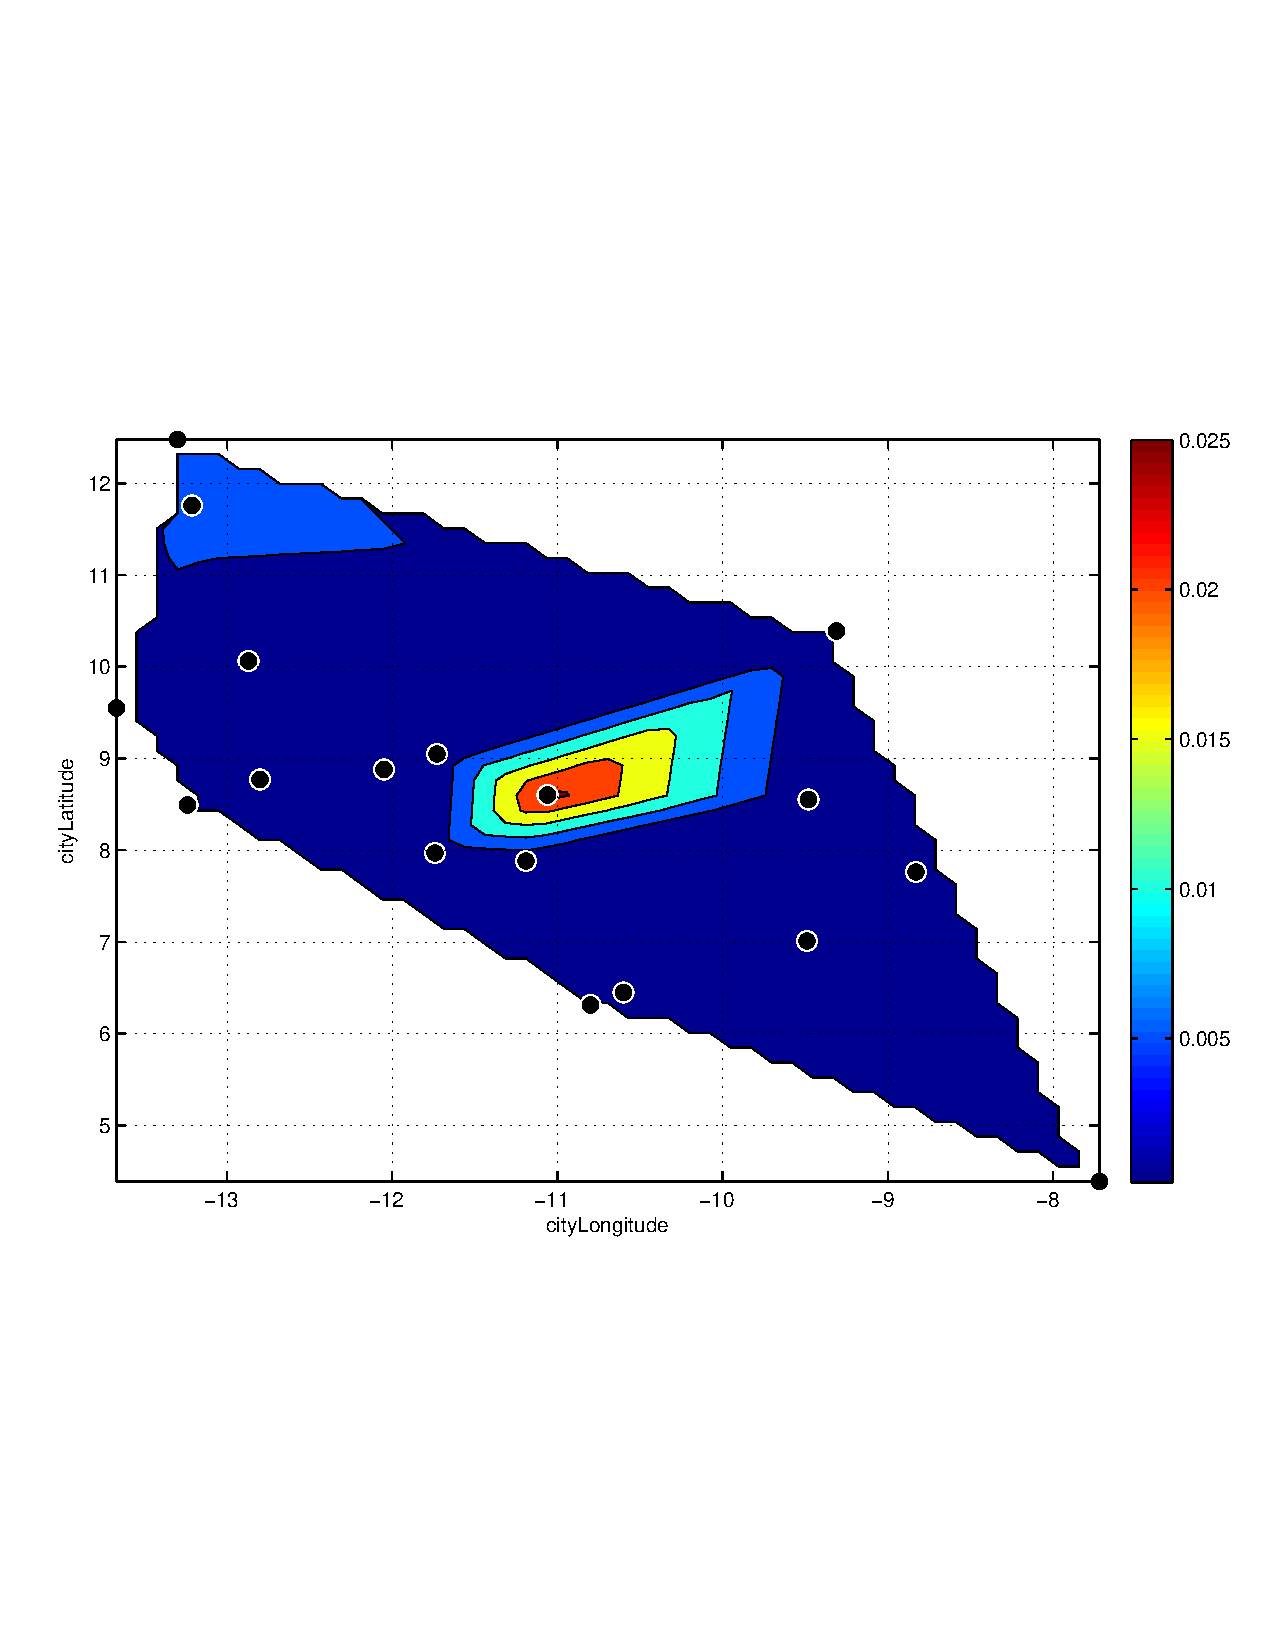
\includegraphics[width=0.6\textwidth]{vaccine_per_capita.pdf}
%\caption{The contour plot of vaccine per capita. The black spots represent locations of the 18 cities.}
%\label{vaccine_per_capita.pdf}
%\end{figure}
%
%\begin{table}[]
%\centering
%\begin{tabular}{|r|r|r|r|}
%\hline
%label of city&$drug_i$&population of city & drug per capita ($\times 10^{-3}$)\\ \hline
%1&32&33190&0.9497\\ \hline
%2&111&167100&0.6643\\ \hline
%3&113&3222&34.9531\\ \hline
%4&93&1548000&0.060143\\ \hline
%5&112&772900&0.14476\\ \hline
%6&76&7461&10.1765\\ \hline
%7&59&45840&1.2819\\ \hline
%8&37&32660&1.1336\\ \hline
%9&14&114000&0.12545\\ \hline
%10&107&137700&0.78005\\ \hline
%11&31&117100&0.26779\\ \hline
%12&1&13990&0.077239\\ \hline
%13&6&43100&0.1433\\ \hline
%14&57&85020&0.67318\\ \hline
%15&108&1011000&0.10657\\ \hline
%16&22&1870&11.6608\\ \hline
%17&9&132700&0.067749\\ \hline
%18&12&21960&0.54899\\ \hline
%\end{tabular}
%\caption{A optimized plan for allocating drug with $drug_{tot} = 1800$ }
%\label{drug}
%\end{table}
